% Options for packages loaded elsewhere
\PassOptionsToPackage{unicode}{hyperref}
\PassOptionsToPackage{hyphens}{url}
%
\documentclass[
]{book}
\usepackage{amsmath,amssymb}
\usepackage{iftex}
\ifPDFTeX
  \usepackage[T1]{fontenc}
  \usepackage[utf8]{inputenc}
  \usepackage{textcomp} % provide euro and other symbols
\else % if luatex or xetex
  \usepackage{unicode-math} % this also loads fontspec
  \defaultfontfeatures{Scale=MatchLowercase}
  \defaultfontfeatures[\rmfamily]{Ligatures=TeX,Scale=1}
\fi
\usepackage{lmodern}
\ifPDFTeX\else
  % xetex/luatex font selection
\fi
% Use upquote if available, for straight quotes in verbatim environments
\IfFileExists{upquote.sty}{\usepackage{upquote}}{}
\IfFileExists{microtype.sty}{% use microtype if available
  \usepackage[]{microtype}
  \UseMicrotypeSet[protrusion]{basicmath} % disable protrusion for tt fonts
}{}
\makeatletter
\@ifundefined{KOMAClassName}{% if non-KOMA class
  \IfFileExists{parskip.sty}{%
    \usepackage{parskip}
  }{% else
    \setlength{\parindent}{0pt}
    \setlength{\parskip}{6pt plus 2pt minus 1pt}}
}{% if KOMA class
  \KOMAoptions{parskip=half}}
\makeatother
\usepackage{xcolor}
\usepackage{longtable,booktabs,array}
\usepackage{calc} % for calculating minipage widths
% Correct order of tables after \paragraph or \subparagraph
\usepackage{etoolbox}
\makeatletter
\patchcmd\longtable{\par}{\if@noskipsec\mbox{}\fi\par}{}{}
\makeatother
% Allow footnotes in longtable head/foot
\IfFileExists{footnotehyper.sty}{\usepackage{footnotehyper}}{\usepackage{footnote}}
\makesavenoteenv{longtable}
\usepackage{graphicx}
\makeatletter
\def\maxwidth{\ifdim\Gin@nat@width>\linewidth\linewidth\else\Gin@nat@width\fi}
\def\maxheight{\ifdim\Gin@nat@height>\textheight\textheight\else\Gin@nat@height\fi}
\makeatother
% Scale images if necessary, so that they will not overflow the page
% margins by default, and it is still possible to overwrite the defaults
% using explicit options in \includegraphics[width, height, ...]{}
\setkeys{Gin}{width=\maxwidth,height=\maxheight,keepaspectratio}
% Set default figure placement to htbp
\makeatletter
\def\fps@figure{htbp}
\makeatother
\setlength{\emergencystretch}{3em} % prevent overfull lines
\providecommand{\tightlist}{%
  \setlength{\itemsep}{0pt}\setlength{\parskip}{0pt}}
\setcounter{secnumdepth}{5}
\usepackage{booktabs}
\ifLuaTeX
  \usepackage{selnolig}  % disable illegal ligatures
\fi
\usepackage[]{natbib}
\bibliographystyle{plainnat}
\usepackage{bookmark}
\IfFileExists{xurl.sty}{\usepackage{xurl}}{} % add URL line breaks if available
\urlstyle{same}
\hypersetup{
  pdftitle={GTI - Banco de dados - 2025 - Anotações de aula},
  pdfauthor={Professor Miguél Suares},
  hidelinks,
  pdfcreator={LaTeX via pandoc}}

\title{GTI - Banco de dados - 2025 - Anotações de aula}
\author{Professor Miguél Suares}
\date{2025-08-04}

\begin{document}
\maketitle

{
\setcounter{tocdepth}{1}
\tableofcontents
}
\chapter*{Sobre estas anotações}\label{sobre-estas-anotauxe7uxf5es}
\addcontentsline{toc}{chapter}{Sobre estas anotações}

---------------------------------------------------------------------------------------------------------------------------------------

Estas anotações são apenas lembretes das aulas expostas em sala, durante a disciplina de Banco de dados.

\section{ACESSO AO GITBOOK CELULAR}\label{acesso-ao-gitbook-celular}

---------------------------------------------------------------------------------------------------------------------------------------

\subsubsection{\texorpdfstring{\url{https://miguel7penteado.github.io/2025-2sem-GTI-BancoDeDados}}{https://miguel7penteado.github.io/2025-2sem-GTI-BancoDeDados}}\label{httpsmiguel7penteado.github.io2025-2sem-gti-bancodedados}


\includegraphics{images/qr-code-disciplina.jpg}

\section{Leitores de formato de arquivo EPUB para SmartPhone}\label{leitores-de-formato-de-arquivo-epub-para-smartphone}

---------------------------------------------------------------------------------------------------------------------------------------

\subsection{ANDROID}\label{android}

\subsubsection{\texorpdfstring{\textbf{Moon+ Reader}}{Moon+ Reader}}\label{moon-reader}


\includegraphics[width=3.54167in,height=\textheight]{images/qrcode/leitor_epub/MoonReaderPlus.jpg}

\section{Livros Texto da Disciplina}\label{livros-texto-da-disciplina}

---------------------------------------------------------------------------------------------------------------------------------------

\subsection{\texorpdfstring{\href{https://www.kufunda.net/publicdocs/Introdu\%C3\%A7\%C3\%A3o\%20a\%20Sistemas\%20de\%20Bancos\%20de\%20Dados\%20(C.\%20J.\%20Date)\%20(z-lib.org).pdf}{``Introdução a sistemas de bancos de dados'' do autor ``\textbf{Christopher John Date}''}}{``Introdução a sistemas de bancos de dados'' do autor ``Christopher John Date''}}\label{introduuxe7uxe3o-a-sistemas-de-bancos-de-dados-do-autor-christopher-john-date}

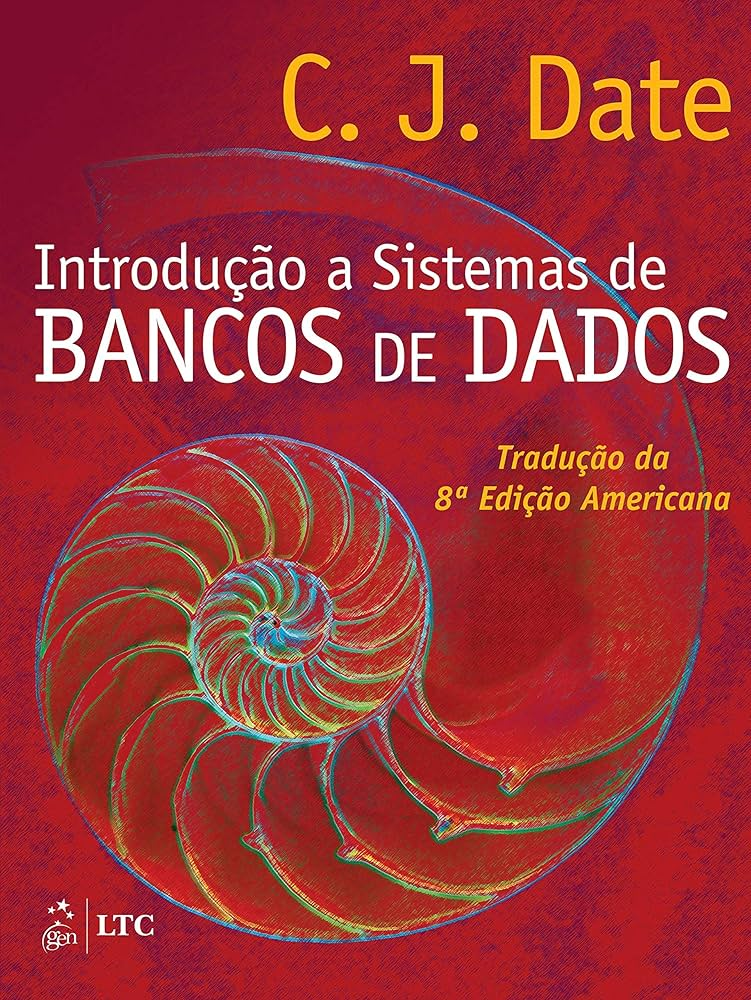
\includegraphics{images/livros/livro1.jpg}

\begin{longtable}[]{@{}
  >{\raggedright\arraybackslash}p{(\columnwidth - 2\tabcolsep) * \real{0.2202}}
  >{\raggedright\arraybackslash}p{(\columnwidth - 2\tabcolsep) * \real{0.7798}}@{}}
\toprule\noalign{}
\endhead
\bottomrule\noalign{}
\endlastfoot
\textbf{Autor(es)} & \begin{minipage}[t]{\linewidth}\raggedright
\subsection{\texorpdfstring{\href{https://en.wikipedia.org/wiki/Christopher_J._Date}{\textbf{Christopher John Date}}}{Christopher John Date}}\label{christopher-john-date}
\end{minipage} \\
\textbf{Editora} & LTC \\
\textbf{Idioma} & Português \\
\textbf{ISBN} & 978-85-352-8445-4 \\
\textbf{Formato} & Capa dura \\
\textbf{Páginas} & 1623 \\
\textbf{Código Biblioteca} & \\
\end{longtable}

\subsection{\texorpdfstring{\href{https://drive.google.com/file/d/0B452rmbcudPSVFdCZ09vVkJUUUd2dlpMNS1vaEczUQ/view?pli=1&resourcekey=0-3MTcHlAYjPX6YSvBQGweUQ}{``\textbf{Projeto de bancos de dados}'' do autor ``Carlos Alberto HEUSER''}}{``Projeto de bancos de dados'' do autor ``Carlos Alberto HEUSER''}}\label{projeto-de-bancos-de-dados-do-autor-carlos-alberto-heuser}

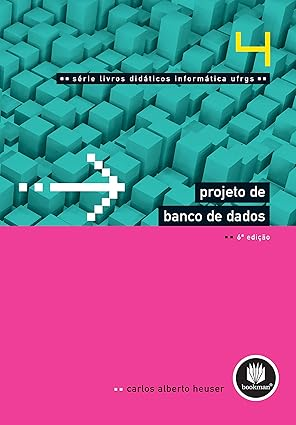
\includegraphics{images/livros/livro2.jpg}

\begin{longtable}[]{@{}
  >{\raggedright\arraybackslash}p{(\columnwidth - 2\tabcolsep) * \real{0.2069}}
  >{\raggedright\arraybackslash}p{(\columnwidth - 2\tabcolsep) * \real{0.7931}}@{}}
\toprule\noalign{}
\endhead
\bottomrule\noalign{}
\endlastfoot
\textbf{Autor(es)} & \begin{minipage}[t]{\linewidth}\raggedright
\subsection{\texorpdfstring{\href{https://www.inf.ufrgs.br/site/docente/carlos-alberto-heuser/}{Carlos Alberto HEUSER}}{Carlos Alberto HEUSER}}\label{carlos-alberto-heuser}
\end{minipage} \\
\textbf{Editora} & Bookman \\
\textbf{Idioma} & Português \\
\textbf{ISBN-10} & 8577803821 \\
\textbf{Formato} & Impresso \\
\textbf{Páginas} & 282 \\
\textbf{Código Biblioteca} & \\
\end{longtable}

\section{Calendário das aulas}\label{calenduxe1rio-das-aulas}

---------------------------------------------------------------------------------------------------------------------------------------

\paragraph{AGOSTO DE 2025}\label{agosto-de-2025}

\begin{longtable}[]{@{}llll@{}}
\toprule\noalign{}
Data & Dia da Semana & Aulas & Conteúdo \\
\midrule\noalign{}
\endhead
\bottomrule\noalign{}
\endlastfoot
04/08/2025 & Segunda-Feira & Aula Inaugural & \\
11/08/2025 & Segunda-Feira & Aula 2 & \\
18/08/2025 & Segunda-Feira & Aula 3 & \\
25/08/2025 & Segunda-Feira & Aula 4 & \\
\end{longtable}

\paragraph{SETEMBRO DE 2025}\label{setembro-de-2025}

\begin{longtable}[]{@{}llll@{}}
\toprule\noalign{}
Data & Dia da Semana & Aulas & Conteúdo \\
\midrule\noalign{}
\endhead
\bottomrule\noalign{}
\endlastfoot
01/09/2025 & Segunda-Feira & Aula 5 & \\
08/09/2025 & Segunda-Feira & Aula 6 & \\
15/09/2025 & Segunda-Feira & NP1 & PROVA \\
22/09/2025 & Segunda-Feira & Aula 7 & \\
29/09/2025 & Segunda-Feira & Aula 8 & \\
\end{longtable}

\paragraph{OUTUBRO DE 2025}\label{outubro-de-2025}

\begin{longtable}[]{@{}llll@{}}
\toprule\noalign{}
Data & Dia da Semana & Aulas & Conteúdo \\
\midrule\noalign{}
\endhead
\bottomrule\noalign{}
\endlastfoot
06/10/2025 & Segunda-Feira & Aula 9 & \\
13/10/2025 & Segunda-Feira & Aula 10 & \\
20/10/2025 & Segunda-Feira & Aula 11 & \\
27/10/2025 & Segunda-Feira & Aula 12 & \\
\end{longtable}

\paragraph{NOVEMBRO DE 2025}\label{novembro-de-2025}

\begin{longtable}[]{@{}llll@{}}
\toprule\noalign{}
Data & Dia da Semana & Aulas & Conteúdo \\
\midrule\noalign{}
\endhead
\bottomrule\noalign{}
\endlastfoot
03/11/2025 & Segunda-Feira & NP2 & PROVA \\
10/11/2025 & Segunda-Feira & & N/A \\
17/11/2025 & Segunda-Feira & SUB & PROVA \\
24/11/2025 & Segunda-Feira & & N/A \\
\end{longtable}

\paragraph{DEZEMBRO DE 2025}\label{dezembro-de-2025}

\begin{longtable}[]{@{}llll@{}}
\toprule\noalign{}
Data & Dia da Semana & Aulas & Conteúdo \\
\midrule\noalign{}
\endhead
\bottomrule\noalign{}
\endlastfoot
01/12/2025 & Segunda-Feira & & N/A \\
08/12/2025 & Segunda-Feira & EXAME & PROVA \\
15/12/2025 & Segunda-Feira & & N/A \\
\end{longtable}

\section{Alunos 2025 - 2o Semestre}\label{alunos-2025---2o-semestre}

---------------------------------------------------------------------------------------------------------------------------------------

\subsection{Campus Chácara Santo Antônio}\label{campus-chuxe1cara-santo-antuxf4nio}

\subsubsection{Turma TI2P40}\label{turma-ti2p40}

\begin{longtable}[]{@{}cc@{}}
\toprule\noalign{}
Matrícula & Nome do aluno \\
\midrule\noalign{}
\endhead
\bottomrule\noalign{}
\endlastfoot
F362BF0 & BRUNO ANTONIO MARQUES \\
R536FA6 & CAIO CESAR BALBINO DA SILVA \\
H6094I1 & DOUGLAS VINICIUS M DOS SANTOS \\
R6607G5 & GABRIEL ROQUE DOS SANTOS \\
R8133G7 & ÍTALO KEVIN RODRIGUES DA SILVA \\
R837AA0 & LUCAS SOUZA RODRIGUES \\
H714419 & MARCOS PAULO CORDEIRO GOES \\
\end{longtable}

\chapter{Aula Inaugural}\label{aula-inaugural}

\subsubsection*{04/08/2025}\label{section}
\addcontentsline{toc}{subsubsection}{04/08/2025}

\subsubsection*{Professor Miguél Suares}\label{professor-miguuxe9l-suares}
\addcontentsline{toc}{subsubsection}{Professor Miguél Suares}

\section{\texorpdfstring{Disciplina: \textbf{Banco de Dados}}{Disciplina: Banco de Dados}}\label{disciplina-banco-de-dados}

\begin{itemize}
\tightlist
\item
  Curso: Gestão em Tecnologia da Informação (GTI)\\
\item
  Período: \textbf{Noturno}\\
\item
  Turma: \textbf{2º semestre de 2025}
\item
  Campus: \textbf{Chácara Santo Antônio}
\end{itemize}

\begin{quote}
``Dados são o novo petróleo.'' -- Clive Humby
\end{quote}

\begin{center}\rule{0.5\linewidth}{0.5pt}\end{center}

\chapter{👨‍🏫 Sobre o Professor}\label{sobre-o-professor}

\begin{itemize}
\tightlist
\item
  Nome: Prof.~Miguél Suares
\item
  Formação: Mestre em Engenharia da Computação e Energia da Agricultura
\item
  Experiência: +10 anos com bancos de dados relacionais e análise de dados
\item
  Contato: \href{mailto:miguel.penteado@docente.unip.br}{\nolinkurl{miguel.penteado@docente.unip.br}}
\end{itemize}

\begin{center}\rule{0.5\linewidth}{0.5pt}\end{center}

\chapter{🎯 Objetivos da Disciplina}\label{objetivos-da-disciplina}

\begin{itemize}
\tightlist
\item
  Compreender os fundamentos de bancos de dados
\item
  Modelar dados com diagramas ER
\item
  Implementar e consultar bases de dados com SQL
\item
  Utilizar ferramentas como MySQL, PostgreSQL, QGIS e R
\item
  Desenvolver raciocínio lógico para resolver problemas com dados
\end{itemize}

\begin{center}\rule{0.5\linewidth}{0.5pt}\end{center}

\chapter{📅 Calendário da Disciplina}\label{calenduxe1rio-da-disciplina}

\begin{longtable}[]{@{}lll@{}}
\toprule\noalign{}
Data & Aula & Tema \\
\midrule\noalign{}
\endhead
\bottomrule\noalign{}
\endlastfoot
04/08/2025 & Aula 1 & Aula Inaugural \\
11/08/2025 & Aula 2 & Fundamentos \\
18/08/2025 & Aula 3 & Modelagem e Diagramas \\
25/08/2025 & Aula 4 & Administração e Gerenciamento \\
01/09/2025 & Aula 5 & Aplicação CRUD \\
08/09/2025 & Aula 6 & MySQL \\
15/09/2025 & \textbf{NP1} & \textbf{Prova} \\
22/09/2025 & Aula 7 & Postgres \\
29/09/2025 & Aula 8 & QGIS \\
06/10/2025 & Aula 9 & RStudio \\
13/10/2025 & Aula 10 & Análise I \\
20/10/2025 & Aula 11 & Análise II \\
27/10/2025 & Aula 12 & Análise III \\
03/11/2025 & \textbf{NP2} & \textbf{Prova} \\
\end{longtable}

\begin{center}\rule{0.5\linewidth}{0.5pt}\end{center}

\chapter{📚 Ementa Resumida}\label{ementa-resumida}

\begin{itemize}
\tightlist
\item
  Introdução a bancos de dados relacionais (RDBMS)
\item
  Modelagem de dados (M.E.R.) e diagramas Entidade Relacionamento (D.E.R.)
\item
  Linguagem SQL: DDL, DML, DCL
\item
  Ferramentas: MySQL, PostgreSQL
\item
  Visualização geoespacial (QGIS)
\item
  Análise e exploração de dados (R e RStudio)
\end{itemize}

\begin{center}\rule{0.5\linewidth}{0.5pt}\end{center}

\chapter{📝 Avaliação}\label{avaliauxe7uxe3o}

\begin{itemize}
\tightlist
\item
  \textbf{Provas (NP1 + NP2)}
\item
  \textbf{Prova Substitutiva}
\item
  \textbf{Exame}
\end{itemize}

\begin{center}\rule{0.5\linewidth}{0.5pt}\end{center}

\chapter{🛠️ Ferramentas da Disciplina}\label{ferramentas-da-disciplina}

\begin{itemize}
\tightlist
\item
  \textbf{Servidores de Banco de Dados}: MySQL, PostgreSQL
\item
  \textbf{Clientes de Banco de Dados}: pgAdmin, MySQL Workbench, DBeaver\\
\item
  \textbf{Geoprocessamento}: QGIS\\
\item
  \textbf{Análise de Dados}: R + RStudio\\
\item
  \textbf{Versionamento e Organização}: GitHub, Teams
\end{itemize}

\begin{center}\rule{0.5\linewidth}{0.5pt}\end{center}

\chapter{📌 Expectativas e Regras}\label{expectativas-e-regras}

\begin{itemize}
\tightlist
\item
  Pontualidade e entrega de atividades no prazo
\item
  Trabalhos devem ser originais (sem plágio)
\item
  Participação ativa nas discussões e práticas
\item
  Uso responsável das ferramentas
\item
  Respeito e colaboração entre colegas
\end{itemize}

\begin{center}\rule{0.5\linewidth}{0.5pt}\end{center}

\chapter{💡 Dicas para Mandar Bem}\label{dicas-para-mandar-bem}

\begin{itemize}
\tightlist
\item
  Faça os exercícios logo após a aula
\item
  Participe das práticas com base real
\item
  Mantenha o repositório do projeto atualizado
\item
  Refaça consultas SQL até entender
\item
  Teste e documente suas soluções
\end{itemize}

\begin{center}\rule{0.5\linewidth}{0.5pt}\end{center}

\chapter{🙌 Encerramento}\label{encerramento}

\section{Estamos prontos?}\label{estamos-prontos}

📧 Dúvidas? Estou à disposição\\
📊 Vamos construir conhecimento juntos!

\begin{quote}
Próxima aula: \textbf{Fundamentos de Banco de Dados} -- 11/08/2025
\end{quote}

\chapter{Fundamentos de Sistemas de Bancos de Dados}\label{fundamentos-de-sistemas-de-bancos-de-dados}

\subsubsection*{11/08/2025}\label{section-1}
\addcontentsline{toc}{subsubsection}{11/08/2025}

\subsubsection*{Professor Miguél Suares}\label{professor-miguuxe9l-suares-1}
\addcontentsline{toc}{subsubsection}{Professor Miguél Suares}

\chapter{Modelagem de Bancos de Dados}\label{modelagem-de-bancos-de-dados}

\subsubsection*{18/08/2025}\label{section-2}
\addcontentsline{toc}{subsubsection}{18/08/2025}

\subsubsection*{Professor Miguél Suares}\label{professor-miguuxe9l-suares-2}
\addcontentsline{toc}{subsubsection}{Professor Miguél Suares}

\chapter{Administração e Gerenciamento de Bancos de Dados}\label{administrauxe7uxe3o-e-gerenciamento-de-bancos-de-dados}

\subsubsection*{25/08/2025}\label{section-3}
\addcontentsline{toc}{subsubsection}{25/08/2025}

\subsubsection*{Professor Miguél Suares}\label{professor-miguuxe9l-suares-3}
\addcontentsline{toc}{subsubsection}{Professor Miguél Suares}

\chapter{Banco de Dados: Uma Aplicação CRUD}\label{banco-de-dados-uma-aplicauxe7uxe3o-crud}

\subsubsection*{01/09/2025}\label{section-4}
\addcontentsline{toc}{subsubsection}{01/09/2025}

\subsubsection*{Professor Miguél Suares}\label{professor-miguuxe9l-suares-4}
\addcontentsline{toc}{subsubsection}{Professor Miguél Suares}

\chapter{Banco de Dados: MySQL (MariaDB)}\label{banco-de-dados-mysql-mariadb}

\subsubsection*{08/09/2025}\label{section-5}
\addcontentsline{toc}{subsubsection}{08/09/2025}

\subsubsection*{Professor Miguél Suares}\label{professor-miguuxe9l-suares-5}
\addcontentsline{toc}{subsubsection}{Professor Miguél Suares}

\chapter{Banco de Dados: Postgres}\label{banco-de-dados-postgres}

\subsubsection*{22/09/2025}\label{section-6}
\addcontentsline{toc}{subsubsection}{22/09/2025}

\subsubsection*{Professor Miguél Suares}\label{professor-miguuxe9l-suares-6}
\addcontentsline{toc}{subsubsection}{Professor Miguél Suares}

\chapter{Banco de Dados Espaciais - Cliente QGIS}\label{banco-de-dados-espaciais---cliente-qgis}

\subsubsection*{29/09/2025}\label{section-7}
\addcontentsline{toc}{subsubsection}{29/09/2025}

\subsubsection*{Professor Miguél Suares}\label{professor-miguuxe9l-suares-7}
\addcontentsline{toc}{subsubsection}{Professor Miguél Suares}

\chapter{Banco de Dados Estatístico - Cliente Rstudio}\label{banco-de-dados-estatuxedstico---cliente-rstudio}

\subsubsection*{06/10/2025}\label{section-8}
\addcontentsline{toc}{subsubsection}{06/10/2025}

\subsubsection*{Professor Miguél Suares}\label{professor-miguuxe9l-suares-8}
\addcontentsline{toc}{subsubsection}{Professor Miguél Suares}

\chapter{Banco de Dados - Análise de Dados Parte 01}\label{banco-de-dados---anuxe1lise-de-dados-parte-01}

\subsubsection*{13/10/2025}\label{section-9}
\addcontentsline{toc}{subsubsection}{13/10/2025}

\subsubsection*{Professor Miguél Suares}\label{professor-miguuxe9l-suares-9}
\addcontentsline{toc}{subsubsection}{Professor Miguél Suares}

\chapter{Banco de Dados - Análise de Dados Parte 02}\label{banco-de-dados---anuxe1lise-de-dados-parte-02}

\subsubsection*{20/10/2025}\label{section-10}
\addcontentsline{toc}{subsubsection}{20/10/2025}

\subsubsection*{Professor Miguél Suares}\label{professor-miguuxe9l-suares-10}
\addcontentsline{toc}{subsubsection}{Professor Miguél Suares}

\chapter{Banco de Dados - Análise de Dados Parte 03}\label{banco-de-dados---anuxe1lise-de-dados-parte-03}

\subsubsection*{27/10/2025}\label{section-11}
\addcontentsline{toc}{subsubsection}{27/10/2025}

\subsubsection*{Professor Miguél Suares}\label{professor-miguuxe9l-suares-11}
\addcontentsline{toc}{subsubsection}{Professor Miguél Suares}

  \bibliography{book.bib}

\end{document}
